\chapter{Conclusions}\label{chap:conclusions}

% **************************** Define Graphics Path **************************
\ifpdf
    \graphicspath{{conclusions/figs/Raster/}{conclusions/figs/PDF/}{conclusions/figs/}}
\else
    \graphicspath{{conclusions/figs/Vector/}{conclusions/figs/}}
\fi

In this thesis, we explored methods for improving the measurement accuracy of radio-frequency receivers for inclusion in the emerging frontier of astrophysics experiments targeting 21-cm hydrogen signatures from the Cosmic Dawn and Epoch of Reionisation. Investigation of these unexamined windows of cosmic history offer new insights into open questions such as the development of structure in the universe \citep{furlanetto_ast}, the nature of dark matter \citep{21cm_dm}, as well as constraints on inflationary theories and spatial curvature \citep{21cm_inflation,21cm_curvature}. With such a broad potential for cosmological insight, analysis of these hydrogen signatures is categorised as an area of scientific importance in the 2020 National Academy of Sciences decadal survey \citep{decade_survey} and has spawned numerous experiments attempting detection including EDGES \citep{edges}, HERA \citep{hera} and the SKA \citep{ska}.

Models for the 21-cm signal, thought to be minute spectral fluctuations redshifted to radio frequencies, are shown to be orders of magnitude smaller than galactic foregrounds \citep{foregrounds}, with terrestrial interference \citep{reach} and even the thermal noise of electronic detection equipment posing a significant challenge to scientific analysis. Such considerations highlight the need for novel instrument design and advanced numerical algorithms to maximise the prospects of experiments. In \cref{chap:instrumentation}, we presented the architecture and construction of a high-quality radio-frequency receiver for deployment in the South African Radio Astronomy Observatory as part of the REACH experiment \citep{reach}. The receiver unit utilises a Dicke switching procedure to mitigate time-variation of the system gain while incorporating up to twelve calibration sources to provide a substantial amount of training data and facilitate the derivation of calibration parameters. A compact design including an onboard VNA, LNA and temperature control system promotes an in situ calibration with automation scripts, crash and backup routines ensuring that the device works with minimal human intervention.

Informing the receiver design was the parallel development of a numerical calibration method named \textsc{Excalibrate}. Based on the noise wave formulation of calibration parameters \citep{meys}, \textsc{Excalibrate} expands on the calibration algorithm developed for the EDGES experiment \citep{edgesCal} by introducing a Bayesian approach to the derivation of these ‘noise wave parameters’. Central to our technique is the utilisation of conjugate priors, giving a closed-form solution for our noise wave parameters and yielding a fast algorithm further promoting characterisation of the instrument in the same environment as the data acquisition--a first of its kind for this type of experiment. Additionally, our procedure incorporates possible correlation between calibration parameters during their derivation and features individual optimisation of parameters which prevents overfitting of the data that may hamper detection of the hydrogen signature.

Our calibration method has been tested with data taken from the REACH receiver at various points of construction as well as with a HERA front end module. In our tests, significant kelvin-level structure were seen in the results despite physical modification to the receiver and, numerical adjustments and revisions of our Bayesian model suggesting that the derivation of calibration parameters as broadband polynomials in frequency may be inadequate for the desired levels of accuracy for modern experiments. Furthermore, results from an independent investigation by the EDGES group seem to corroborate our findings indicating the need for an alternative approach if advancements in calibration technology are to continue \citep{murray_calpap}.

Following these findings, additional tests were conducted using a separate procedure employing a least squares algorithm to determine the noise wave parameters on a frequency-by-frequency basis which exhibited less chromaticity in the results. We then presented a framework for a Bayesian frequency-by-frequency solver which may be developed to yield a calibration accuracy at the tens-of-millikelvin level.


% =========================================
\section{Future work}\label{sec:future}
As made clear by the results presented in this thesis, there are multiple avenues of further research for increasing instrument sensitivity and accuracy including the development of a more robust numerical calibration algorithm, improvements to the receiver design as well as the continued deployment of the REACH experiment. Our Bayesian pipeline developed in \cref{chap:calibration} currently gives calibration solutions with a variation $\sigma$ around 1 kelvin for 2-minute integrations on the calibration sources. This level of accuracy is however too large to confidently identify the cosmic 21-cm signature believed to have a magnitude up to 250 mK according to theoretical models and up to 500 mK if the EDGES results can be confirmed \citep{theory_models,edgesNature}. Although we have suggested continued work on a frequency-by-frequency solver, the 500 mK accuracy achieved by the precursor MATLAB algorithm still contains too much noise to make a detection.

A more advanced procedure was developed where power and reflection measurements are submitted to a simulation based inference algorithm to learn corresponding calibrator temperatures following a neural ratio estimator framework. Once trained, input of the antenna measurements would ideally give a calibrated temperature probability distribution. It was seen however that the software did not generalise to higher temperatures like the antenna leading to unsatisfactory results. Improvements to the technique are anticipated which will attempt to learn $g$ and $\T{rec}$ instead as these values are expected to be more stable across measurements\footnote{Contact Dr. Harry Bevins (htjb2@cam.ac.uk) for more information.}. We do recommend that caution be taken with such approaches based on neural networks as the solution may open an interpretability issue when reporting results \citep{bb_interpret}.

Another potential subject of continued investigation is the inclusion of a more advanced noise model in our pipeline. Currently, we assume that the noise on calibration measurements is Gaussian and uncorrelated which may not be true. It may be reasonable to expect that noise in neighbouring frequency bins is correlated which diminishes at frequency bins that become increasingly distant. We certainly see empirically that non-ideal behaviour increases with decreasing wavelength which is typical in RF applications. Inclusion of a Gaussian process that models this may be beneficial for identifying noise in parameter derivation. As briefly mentioned in \cref{sec:fbf}, stepping away from unregulated priors may also be advantageous.

Spikes from electromagnetic and radio-frequency interference also pose issues in the detection of minute cosmic signals. In the results presented throughout this work, point-like errors were exhibited at precise frequencies which could be excised through typical numerical masking procedures. While a Bayesian RFI flagger has been developed by \citet{sam_rfi}, we also raise concern with the possibility of broadband RFI corrupting the data. This form of interference, which would affect an extended band of frequencies in more subtle ways than spikes present in the data, may be more difficult to identify and remove. Similar issues are under consideration in related experiments such as HERA \citep{hera_rfi}.

As demonstrated in \cref{sec:matlab_avg_results}, continued integration during spectral measurements may also increase calibration accuracy. The extreme example presented in \cref{sec:matlab_avg_results} results from a combined 165 hours of integration which is not very feasible based on the long-term variability of the instrument as well as an obvious disjoint between time spent on calibration measurements versus sky observations. Considerations for how to reduce the time needed on calibration measurements will need to be explored. For instance, the needed levels of averaging and smoothing suggest the employment of a better spectrometer and VNA unit respectively. Much of the time spent on calibration is integration on calibration sources. Implicit in much of this thesis are questions about how many calibrators are needed to provide an adequate set of training data. Historically, measurements of an open or shorted cable were used to determine calibration parameters analogous to our $\T{unc}$, $\T{cos}$ and $\T{sin}$ \citep{rogersCal} with the ambient and heated load providing the main temperature references for the remaining parameters \citep{edgesCal}. As shown by our simulated results in \cref{sec:simulated_data}, constraints on the noise wave parameter posteriors increased with additional calibrators, however each additional calibrator provided diminishing returns with regard to the amount of information gained (see \cref{fig:linearall}. Conversely, a large set of available calibration sources may be beneficial during deployment as described in \cref{sec:matlab_results} where data from two of the calibrators were found to be inconsistent with the remaining data and were thus excluded from the analysis. If it is determined that fewer calibration sources are needed to achieve the desired level of quality in the data, perhaps through some sort of evidence-based comparison, ports on the MS1 switch may be vacated for the S-O-L standards used in VNA calibration which would avoid the need for the S-parameter modelling prescribed in \cref{sec:tparameters}.

Some general areas for consideration include a better grasp of the calibrator temperatures during measurement. As shown in \cref{sec:cable_gradient}, a model accounting for a temperature gradient across the length of the cable-based calibrators was seen to reduce structure in the results. Improvements to the models may need to be made as calibration accuracy increases to incorporate the temperature of connecting structures such as the MS1, MS3 and MS4 powered switches which have their own temperature profile and heat generation due to frequent toggling. While the TC-08 data logger is limited to eight simultaneous measurements, the Teensy 3.5 microcontroller board can accommodate up to 64 I\textsuperscript{2}C temperature probes. This would allow for temperature measurement of each calibrator termination, the mechanical switches as well as on multiple points along the calibrator cable length which may lead to better informed models further improving measurement quality. The correction for the laboratory-based antenna in \cref{sec:ant_corrections} will need to be extended for application to the in-field hexagonal dipole antenna, especially if a device such as a balun is present in the signal chain between the antenna and receiver input. Additionally, models for antenna loss such as those discussed in \citet{rogersCal} may need to be applied following a form similar to:
\begin{equation}
    \T{corrected} = \left( \T{raw} - \T{ambient}(10^{-\frac{l}{10}} - 1) \right) / 10^{-\frac{l}{10}}, 
    \label{eqn:ant_loss}
\end{equation}
where $l$ is the antenna loss in dB including ground loss, resistive loss, transmission line loss and balun loss. Furthermore, some concern has been raised regarding the vitality of the thermal management systems in the desert environment of the Karoo. While the systems were adequate in the Cambridge laboratory, they have not been extensively tested in the field. For extended data acquisition, an increased power budget may be required as the TEC unit contends with the day/night temperature variations as large as 30 \textdegree C \citep{karoo_temp}.

One final area of future work is the continued deployment of the REACH experiment. Currently, the receiver front- and back-ends as well as the hexagonal dipole installed at the deployment site. As detailed in \cref{chap:instrumentation}, the back-end has infrastructure to accommodate multiple antennas connected to independent receiver front-ends. A second receiver front-end is under construction in Cambridge following the specifications presented in this work with little modification. As detailed in \citet{reach}, simulations for a conical log spiral antenna have been completed for deployment following the current antenna-receiver system. Envisioned is an array of three antennas placed in a triangle configuration each connected to the single back-end and solar panel node as shown in \cref{fig:reach_prime}
\begin{figure}
    \centering
    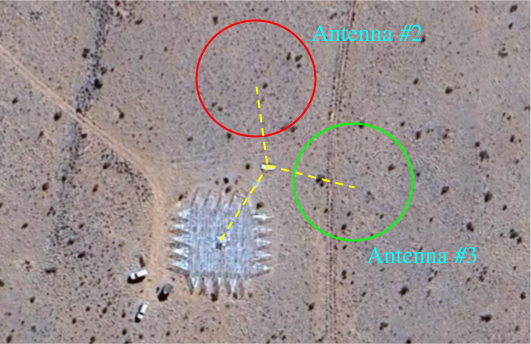
\includegraphics[width=.7\textwidth]{reach_prime}
    \caption{A mock-up of the envisioned REACH experiment with potential sites of future antennas highlighted. Coloured circles represent a reasonable area needed for installation of an antenna along with its ground plane and separate receiver front-end unit. Antenna installations would all be located 100 metres (yellow dashed lines) from the singular recever back-end unit and solar panel array seen at the image's centre. A conical log spiral antenna has been proposed as a second REACH installation. Various options for a third REACH installation are being explored including a scaled antenna for identification of systematics in observation data.}
    \label{fig:reach_prime}
\end{figure}
It is thought that through the use of multiple antennas, redundant systematics and interference may be easily identified and removed. The experiment may also take advantage of the unique features attributed to different antenna designs such as the lower chromatic distortions of the conical log spiral versus the mechanical simplicity of the hexagonal dipole \citep{dom_antenna,john_antenna,reach}. The inclusion of many antennas poses some concerns however such as the possible spawning of antenna crosstalk as present in the HERA experiment \citep{hera_crosstalk} in the form of correlation or interference between the three proposed antennas. Nevertheless, with appropriate precautions in place and a robust calibration routine, the experiment may provide a unique window onto the early universe through the detection of the 21-cm hydrogen signature.

